\begin{knitrout}
\definecolor{shadecolor}{rgb}{0.969, 0.969, 0.969}\color{fgcolor}\begin{figure}

{\centering 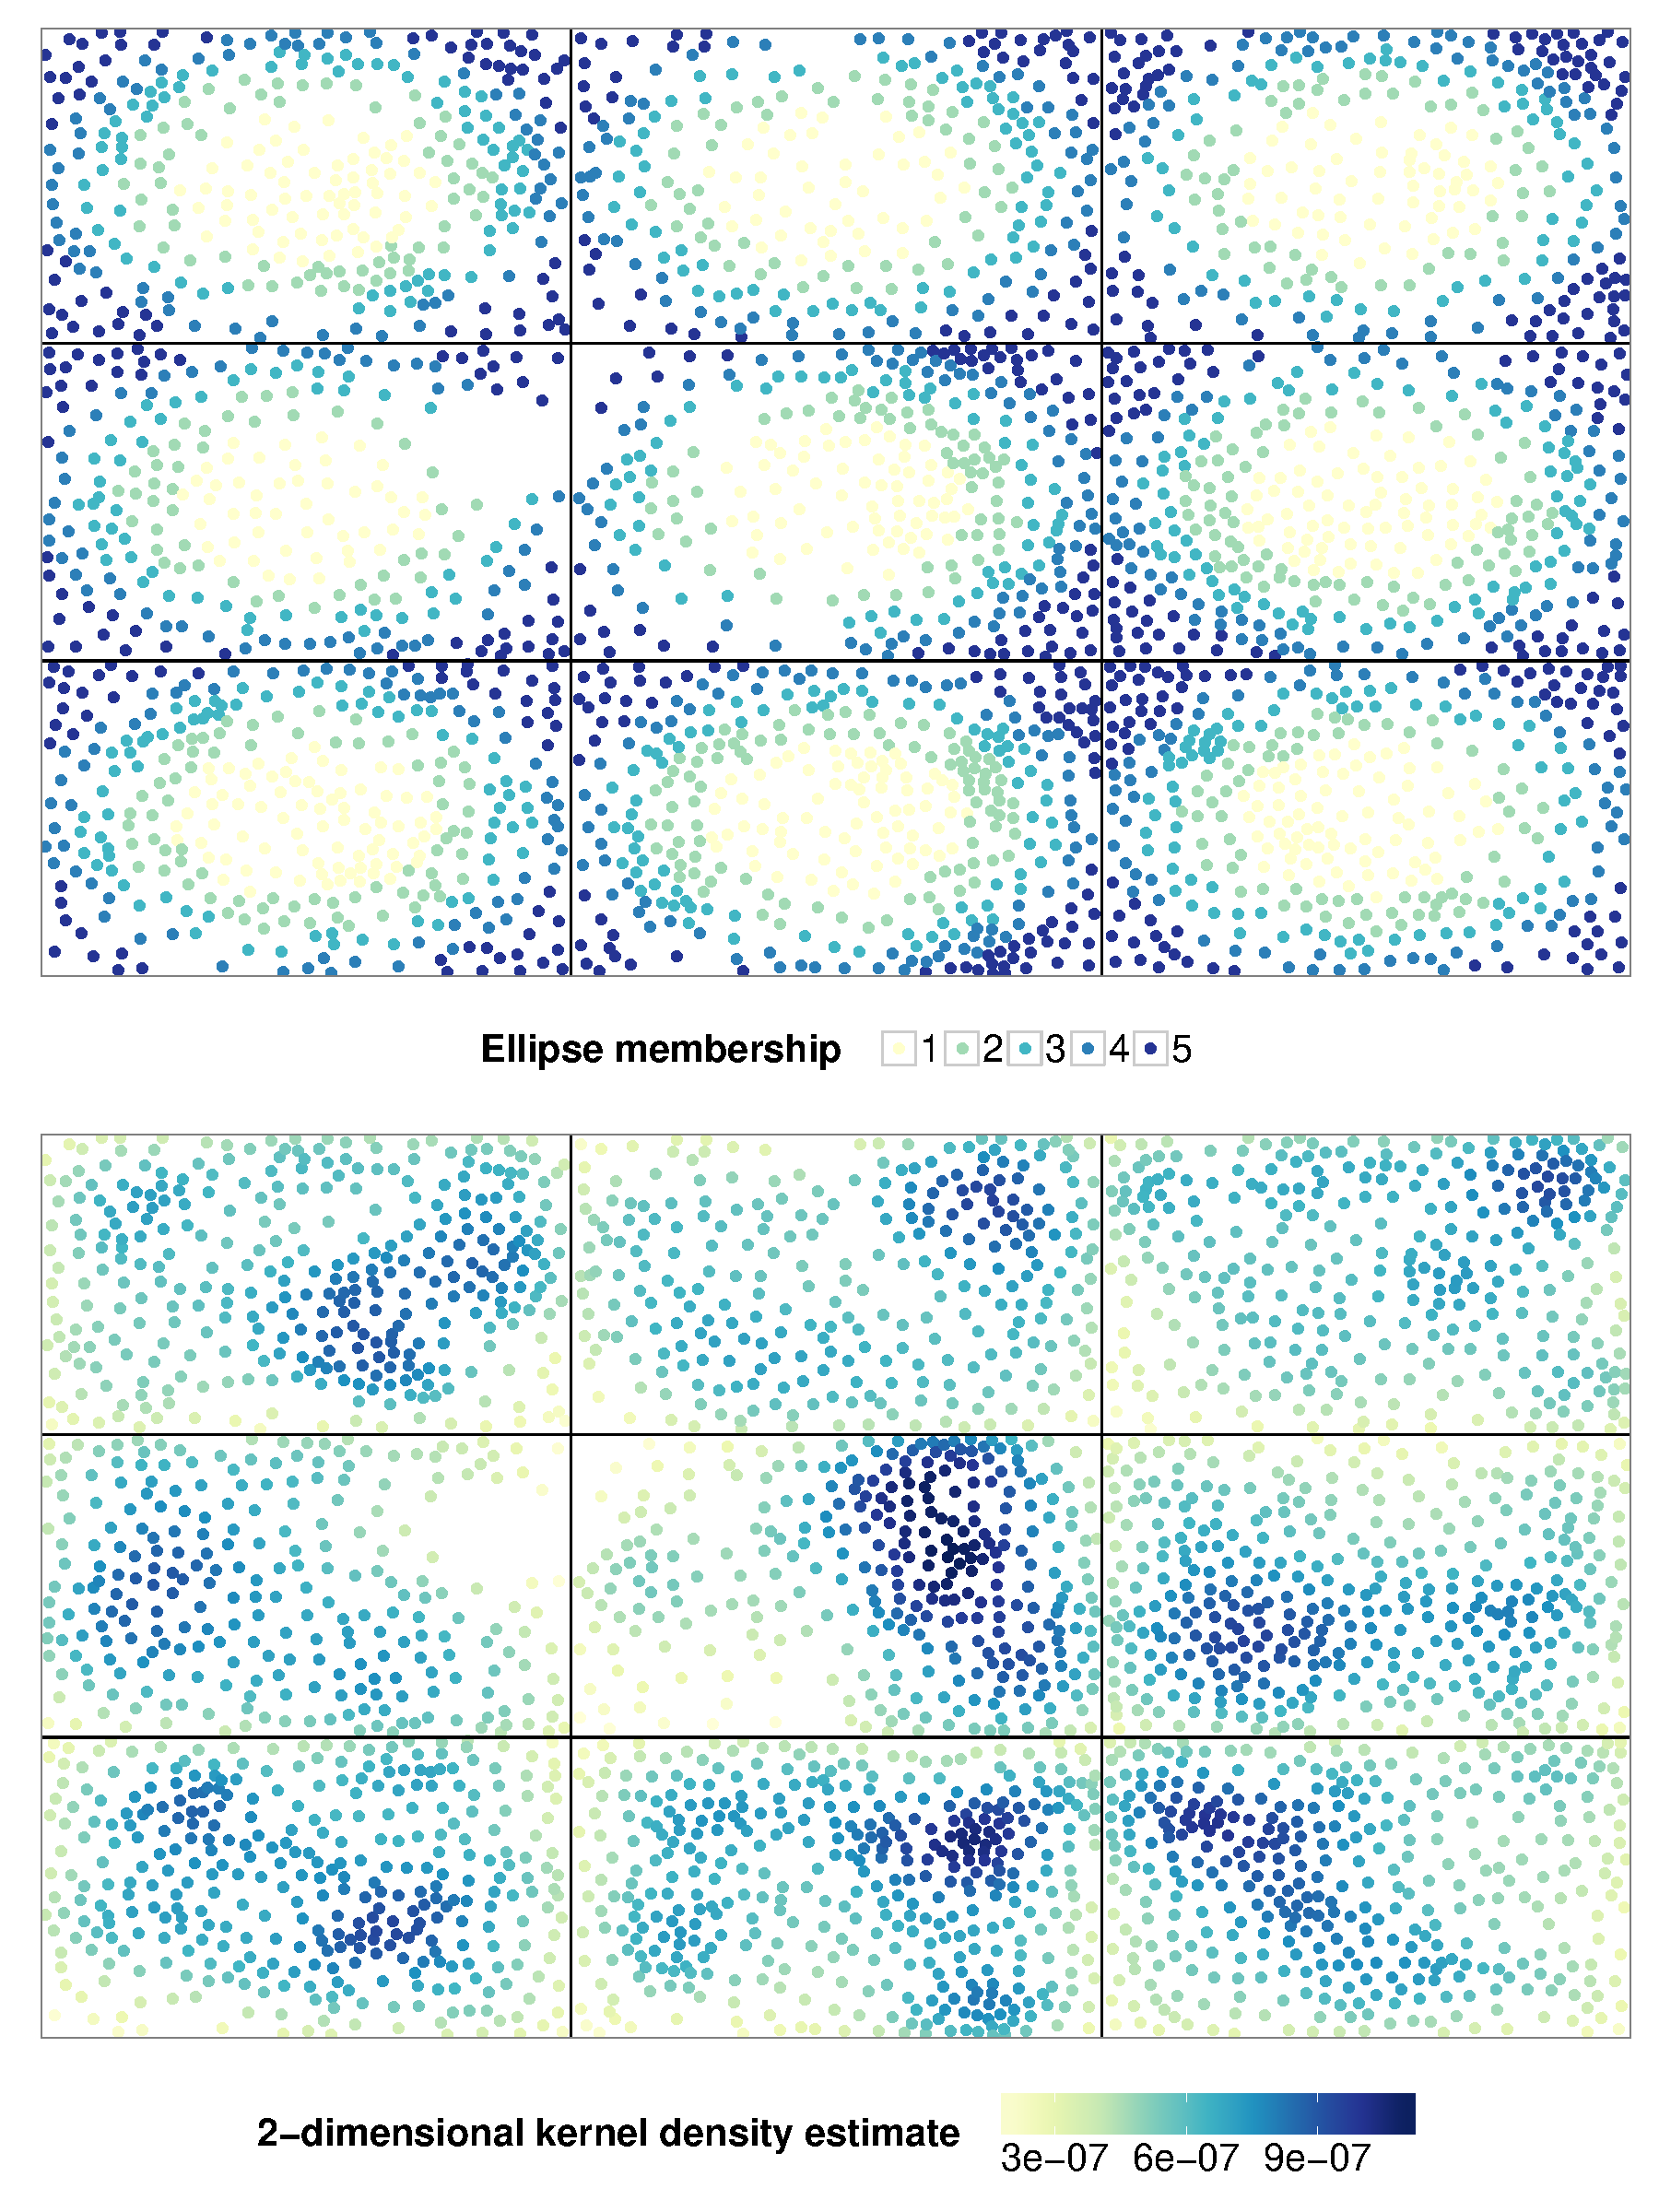
\includegraphics[width=.8\linewidth]{figures/R/augmentationFeatures-scf-augFeat_plot-1} 

}

\caption[Examples of coordinate augmentation functions as implemented in singleCellFeatures.]{Two examples of coorinate augmentation functions aiming at producing useful information from coordinates of cellular objects. The first image shows the discretized elliptic distance (5 bins of equal area) from individual image centers which could be relevant because of deteriorating optical properties of microscope lenses, while the second diagram visualized the 2-dimensional density of cellular objects, an important population context feature. Data is taken from well H6 of plate J107-2C.}\label{fig:scf-augFeat_plot}
\end{figure}


\end{knitrout}
